\documentclass[../main.tex]{subfiles}

\begin{document}
In this section we discuss a voting mechanism, that is an additional layer to secure the consensus against potential attacks. The idea is that nodes query other nodes about their current opinion of the ledger, and adjust their own opinion over the course of several rounds based on the proportion of other opinions they have observed. For this section, we only consider algorithms that find consensus on the value of a single bit, i.e., of a single conflict. The result of this consensus process can then be used to mark a transaction as either \enquote{liked} or \enquote{disliked}.

The general idea is to let the nodes talk to each other in order to resolve the conflicts \textit{pro-actively}. The conflict resolution is performed starting from an initial opinion on the ledger status described as follows:
Consider a transaction $v$. If in a given interval a node does not see any other transaction spent from the same address, we say that the node \textit{likes} transaction $v$; otherwise, the node \textit{dislikes} $v$\footnote{It is important to note, that this rule does not include reattachments: If $v_1,\ldots ,v_k$ are all reattachments of the same transaction, we either like all or none of them.}.
The decision whether a transaction is liked or disliked must then be taken into account for the tip selection.
The most straightforward way of integrating this in any random walk-based TSA is to simply remove the corresponding edges of disliked transactions and, thus, excluding them and any transaction in their future cone from the tip selection.

After that, we periodically apply a voting scheme to every transaction in the Tangle where each node asks for the opinion of some of its neighbors. After the vote, a transaction is either definitely liked or definitely disliked by a node, and this value will never change.
We would like to keep monotonicity in the sense that if a node likes $u$ then it likes any transaction $u$ approves, and if the node dislikes $v$ then it dislikes any transaction that approves $v$, see Figure~\ref{f_voting_consist}.
To achieve this, we can safely assume that we can only like transaction~$v$ when we like all of its past cone, and if we dislike~$v$ then we dislike all of its future cone.

\begin{figure}
\begin{center}
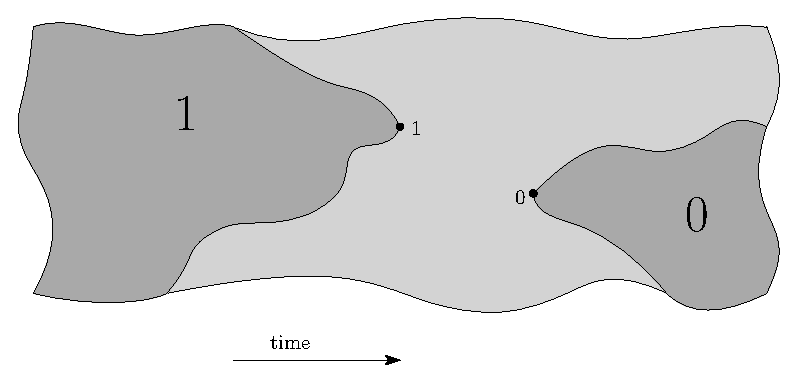
\includegraphics[width=0.75\textwidth]{voting_consist}
\caption{Votes must be consistent}
\label{f_voting_consist}
\end{center}
\end{figure}

In the following two subsections, we will describe two voting mechanisms we are considering.
The first one, called \emph{Fast Probabilistic Consensus}, is certified by rigorous mathematical proofs; however, this solution requires nodes to accept connections from nodes which are not neighbors, and uses decentralized randomness, that needs to be acquired as part of an additional layer.
On the other hand, the cellular automaton approach of Section~\ref{s_cellular} does not have those requirements and seems to be somewhat faster from the first simulations; however, this scheme lacks rigorous proofs and requires a stricter auto peering solution to avoid Eclipse attacks, and formation of \enquote{islands} of adversarial nodes.
The two solutions can be considered as different non-mutually exclusive implementations of the voting mechanism, and they can be used in combination to build a bullet-proof framework.
\end{document}
